\documentclass[12pt,fleqn]{article}\usepackage{../common}
\begin{document}
Karisimlar ve Idare Edilmeyen Kumeleme (Unsupervised Clustering)

Gaussian (normal) dagilimi tek tepesi olan (unimodal) bir dagilimdir. Bu
demektir ki eger birden fazla tepe noktasi olan bir veriyi modellemek
istiyorsak, degisik yaklasimlar kullanmamiz gerekecektir. 

Birden fazla Gaussian'i ``karistirmak (mixing)'' bu tur bir yaklasim
olabilir. Karistirmak, karisim icindeki her Gaussian'dan gelen sonuclari
toplamaktir, yani kelimenin tam anlamiyla her veri noktasini teker teker
karisimdaki tum dagilimlara gecip sonuclari toplamaktir. Eger cok boyutlu
normal dagilimlari topluyorsak, formul:

\[ p(x) = \sum_z \pi_z N(x | \mu_z,\Sigma_z) \]

$\pi_z$ karistirma oranlaridir (mixing proportions). Iki Gaussian oldugunu
dusunelim, oranlar 0.2, 0.8 olabilir mesela (toplam her zaman 1
olmalidir). Karisim oranlarina degisik bir bakis acisini simdi
isleyecegiz. Ornek olarak alttaki grafige bakalim.
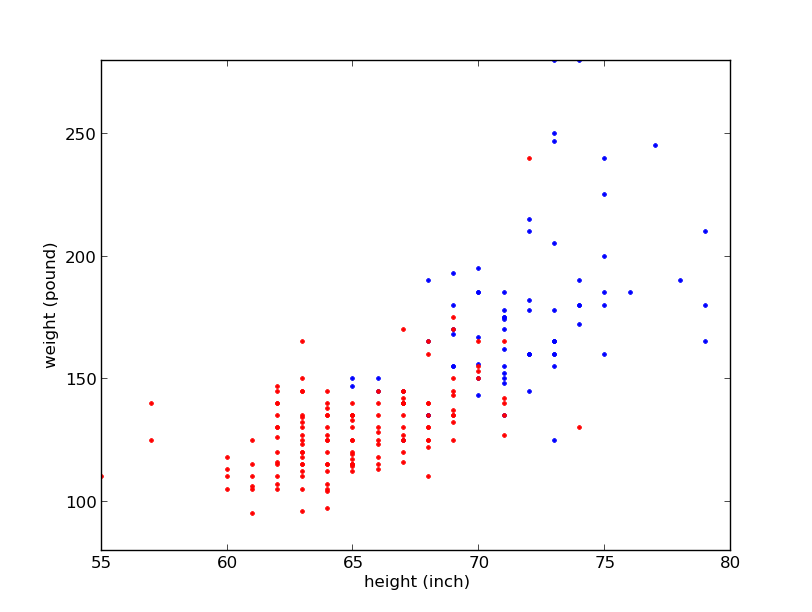
\includegraphics[height=6cm]{plotbio.png}

Bu grafik kadinlar ve erkeklerin boy ve kilolarini iceren bir veri setinden
geliyor, veri setinde erkekler ve kadinlara ait olan olcumler isaretlenmis,
biz de bu isaretleri kullanarak kadinlari kirmizi erkekleri mavi ile
grafikledik. Bu isaretler verilmis olsun ya da olmasin, eger bu veriye bir
dagilim uydurmak (fit) istersek, bir karisim kullanmamiz
gereklidir. Karisimi olusturan Gaussian'lar mesela su sekilde olabilir
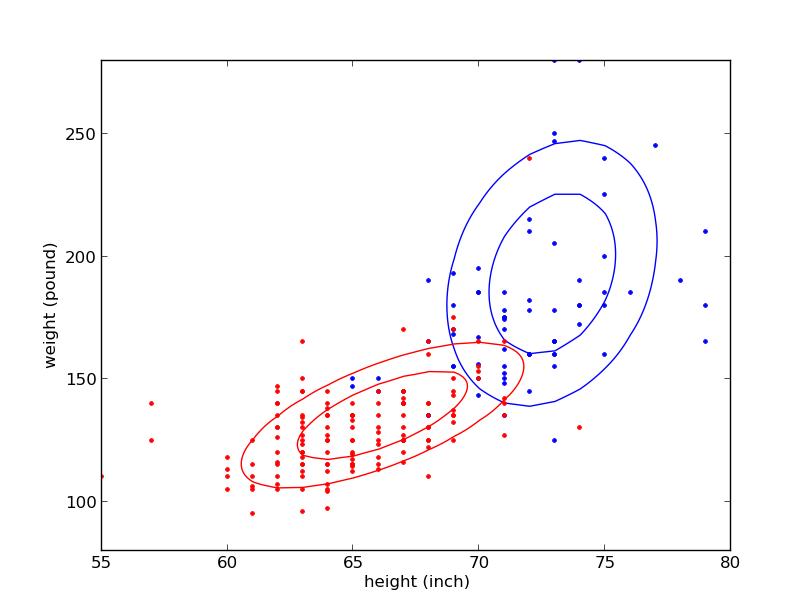
\includegraphics[height=6cm]{plotbio_cluster.png}

Nihai olasilik degeri $p(x)$'i hesaplamak icin her noktayi her iki
Gaussian'a teker teker geceriz, ve sonuclari karisim oranlari ile carparak
toplariz. Kesisme olmayan bolgelerdeki noktalari dusunursek, o noktalarin
olasilik degeri zaten agirlikla tek bir Gaussian'dan geliyor olacak (diger
Gaussian o bolge icin sifira yakin bir deger verecek, bu deger toplamda bir
fark yaratmayacaktir). Kesisim olan bolgelerdeki noktalar ise agirliklara
gore carpilip toplanacak. Agirligi fazla olan Gaussian bu bolgeler icin
anlamli, demek ki o bolgede o Gaussian daha yogun noktalara sahip (bu
yuzden o bolgede daha fazla olasilik veriyor olmasi gerekir). 



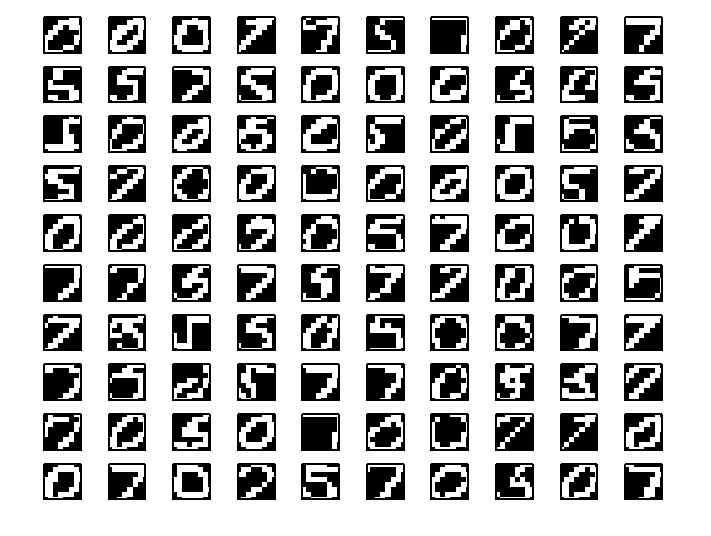
\includegraphics[height=6cm]{digits.png}




\end{document}
